

An interesting question then is
whether the system could extract useful information from seeing an
object manipulated by someone else.  In the case of poking, the robot
needs to be able to estimate the moment of contact and to track the arm
sufficiently well to distinguish it from the object being poked.  We
are interested in how the robot might learn to do this.  One approach
is to chain outwards from an object the robot has poked.  If someone
else moves the object, we can reverse the logic used in poking --
where the motion of the manipulator identified the object -- and
identify a foreign manipulator through its effect on the object.
The next experiment was designed to explore this aspect.


\begin{figure*}[tb]
\begin{center}
%%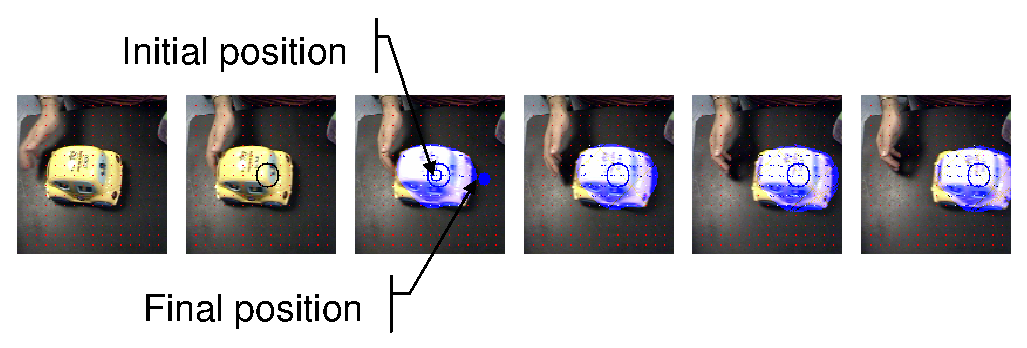
\includegraphics[width=\columnwidth]{observed-action.eps}
\includegraphics[width=\textwidth]{fig-mimicry-bottle}
\caption{ 
\label{fig:observed-action}
%
Basic mimicry.  The first step in mimicking an action is to actually
be able to observe it.  The first sequence shows a human demonstration
of a poking operation.  Frames around the moment of contact are shown.
The object, after segmentation, is tracked for 12 frames using a
combination of template matching and optic flow.  The big circles
represent the tracked position of the bottle in successive frames.
The arrow displayed on the frame of contact ($3^{rd}$ from the left)
projects from the position at the time of contact and at the $12^{th}$
frame respectively.
%
In the second sequence, the bottle is presented to the robot in the
same orientation it had in the demonstrated action and the robot
repeats the observed action, a ``side tap''.  In the third sequence,
the car is presented at a different angle.  The appropriate action to
exploit the affordance and make the bottle roll is now a ``back
slap''.
%
%An example of observed sequence with tracking superimposed. 
%Frames around the
%moment of contact are shown. The object, after segmentation, is tracked for 12 
%frames using a combination of template matching and optic flow. The big circles
%represent the position of the toy car in successive frames. The two small circles
%(outline and solid) displayed on the frame of contact ($3^{rd}$ from the left) are 
%the position at the time of contact and at the $12^{th}$ frame respectively.
%
}
\end{center}
\end{figure*}

The first obvious thing the robot can do is to identify the action just observed 
with respect to its motor vocabulary. It is easily done, in this case, by comparing 
the displacement of the object with the four possible actions and by choosing the
action whose effects are closer to the observed displacement.
Indeed it allows -- even if in this limited setting -- recognizing 
a complex action by interpreting its consequences on the environment.
This is orders of magnitude simpler than trying to completely characterize the
action in terms of the observed kinematics of the movement. Here, the complexity
of the data we need to obtain from the observations is somehow proportional to the complexity
of the goal rather than that of the structure/skills of the foreign manipulator. In our case, because 
the action, the goal, and the object are relatively simple, the only information 
required is about the displacement of the object. 

Therefore, the next question is whether we can use this ``understanding'' of 
observed actions to implement mimicry behavior. It 
would be easy now to try to replicate the action just observed if the same
object were presented again. However, there is still a bit of ambiguity in that
we can choose to mimic either the observed displacement of the object or 
the way the object was poked with respect to its rolling affordance.
 
We chose to implement the latter. It is clear that poking along a particular 
observed direction requires trivial modifications. In practice, after an 
action is observed the angle between the affordance (see table \ref{tab:affordances}) and
the actual displacement is measured and stored. If it happens to see the same 
object again, the robot chooses the action that has the greatest 
probability of poking the object along the previously stored angle. 
Figures \ref{fig:observed-action} and \ref{fig:mimicked-action} show examples of such mimicry.


This response is exactly what we would expect from a ``mirror-type'' representation.
The observed action is interpreted on the basis of the robot own motor code. The same
data structure is also used/activated when performing an action in response to the
sight of a known object. The causal link between the two events that could be separated
by several seconds is the object, the goal, and the object's affordances. There is 
considerable precedent in the literature for a strong connection between viewing 
object manipulation performed by either oneself or another \cite{wohlsclager02human}.
There is also a growing evidence that imitation is goal-directed 
\cite{bekkering-wohlschlager-2000} and that the object of the action is explicitly 
coded (e.g. during reaching) \cite{woodward-1998}.


\begin{figure*}[tb]
\begin{center}
%%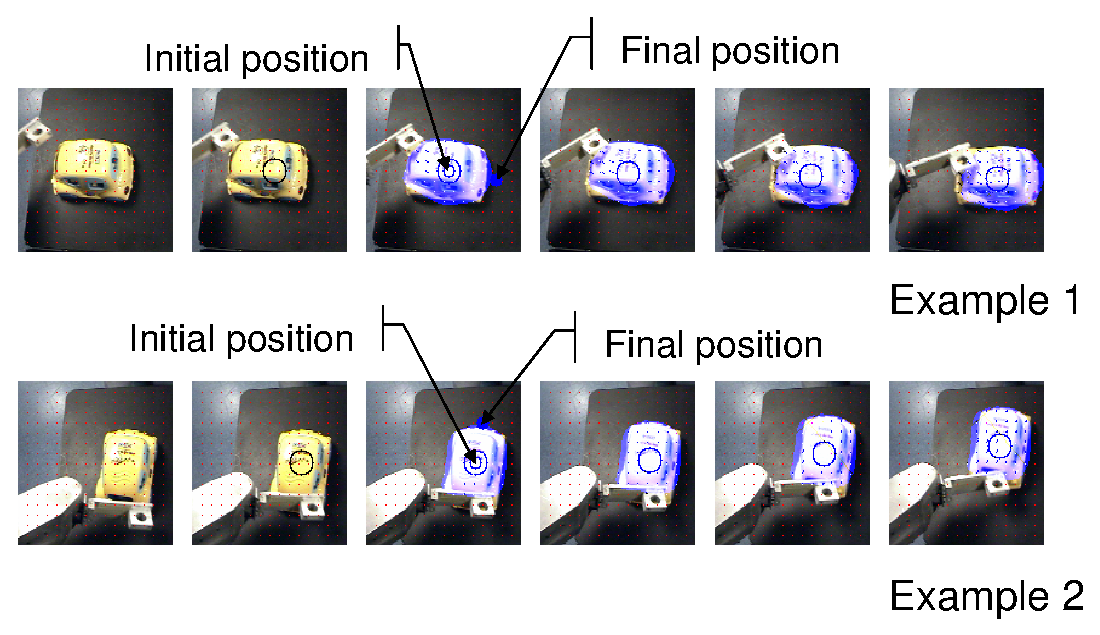
\includegraphics[width=\columnwidth]{mimicked-action.eps}
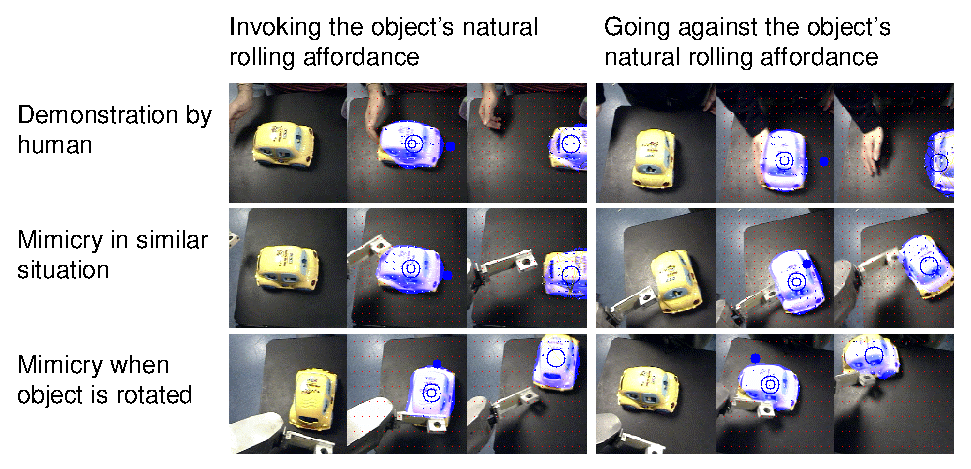
\includegraphics[width=\textwidth]{fig-mimicry-awkward.eps}
\caption{ 
\label{fig:mimicked-action}
%
An extended mimicry example using the toy car.
The sequences on the left show the robot mimicking a human exploiting
the car's rolling affordance.  The sequences on the right show
what happens when the human hits the car in a contrary fashion, going
against its preferred direction of motion.  The robot mimics this 
``unnatural'' action, suppressing its usual behavior of trying to
evoke rolling.
%OUTDATED Two examples of mimicry following the observation in figure \ref{fig:observed-action} 
%where a human manipulator pokes the toy car exploiting the affordance (the car rolls). 
%In example 1 (top row), the toy car has the same orientation it had in the
%demonstrated action and the robot repeats the observed action. In example 2 (bottom), 
%the car is $90^\circ$ with respect to example 1. The appropriate action to exploit
%the affordance and make the car roll is thus a back slap. 
%
}
\end{center}
\end{figure*}


%
\begin{figure}[tb]
\begin{center}
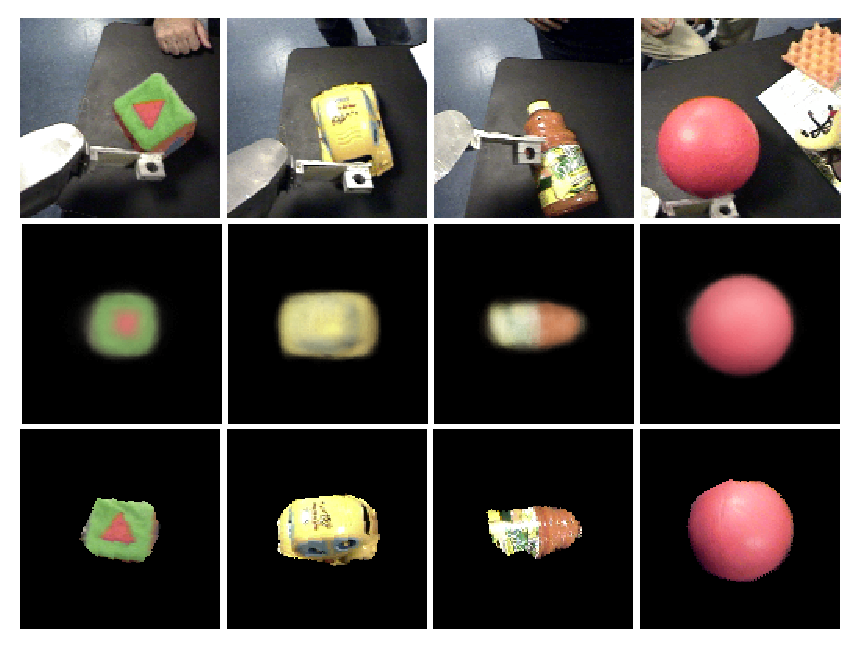
\includegraphics[width=\columnwidth]{fig-auto-proto.eps}
\caption{ 
\label{fig:auto-proto}
%
The top row shows the four objects used in this 
experiment, seen from the robot's perspective.  The 
middle row shows prototypes derived for those objects
using a na\"{\i}ve alignment procedure.  
%All the views
%of a single object (as determined by color histogram
%comparison) were aligned horizontally based on
%their segmentations.  The views were then simply 
%averaged, along with their masks, producing the
%result shown here.  
None of the prototypes contain
any part of the robot's manipulator, or the 
environment.  These prototypes are used 
to find the best available segmentations
of the objects (bottom row).
%
}
\end{center}
\end{figure}



\begin{figure}[tb]
\begin{center}
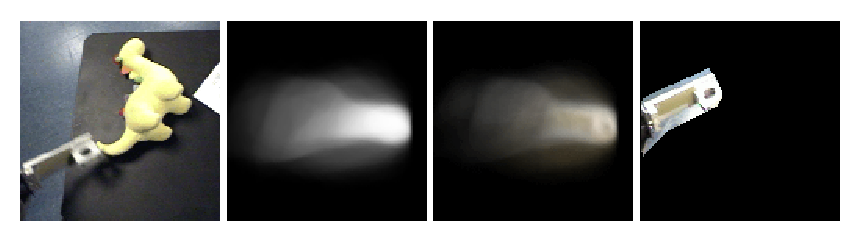
\includegraphics[width=\columnwidth]{fig-auto-proto-flipper.eps}\\
\includegraphics[width=\columnwidth]{fig-auto-proto-hand.eps}
\caption{ 
\label{fig:auto-proto-flipper}
%
The robot manipulator (top left) was automatically segmented during 20
poking sequences.  The segmentations were aligned and averaged, giving
the mask and appearance shown in the adjacent images.  The best
matching view is shown on the top right.  A similar result for the
human hand is shown on the bottom, based on much less data (5 poking
sequences, hands of two individuals).
%BREAK
%The human hand (see left) was automatically segmented during just 5
%poking sequences.  Hands of two different individuals were used.  The
%segmentations were aligned and averaged, giving the mask shown in the
%second image and the mean view shown in the third.  The best matching
%view is shown on the right.  
%Despite the paucity of the data,
%the mean view at least captures skin tone, which is sufficient to
%discard poor segmentations from consideration.
%
}
\end{center}
\end{figure}



\begin{figure}[bt]
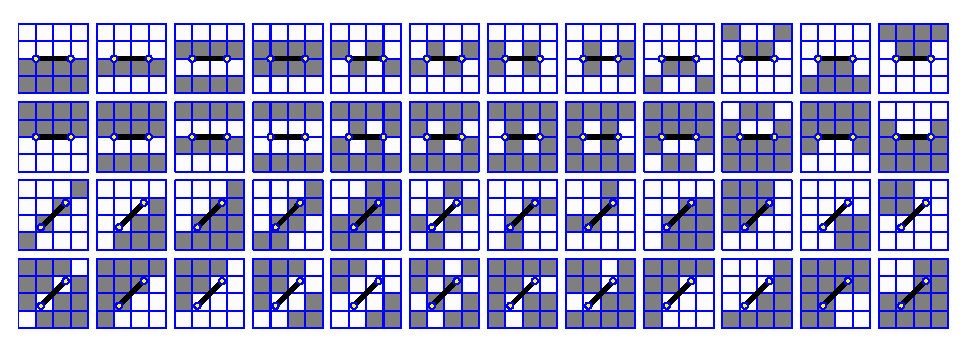
\includegraphics[width=\columnwidth]{seen-selected}
\caption
{
\label{fig:seen-selected}
%
Edges have diverse appearances.  This figure shows 
the orientations assigned to a test suite
prepared by hand.  Each $4\times 4$ grid is a single test
edge patch, and the dark line centered in the grid is the orientation
that patch was observed to have in the training data.
The oriented features represented
include edges, thin lines, thick lines, zig-zags, corners
etc.  It is difficult to imagine a set of conventional
filters that could respond correctly to the full range of 
features seen here~-- all of which appeared multiple
times in object boundaries in real images.
%
}
\end{figure}


\begin{figure}[tb]
\begin{center}
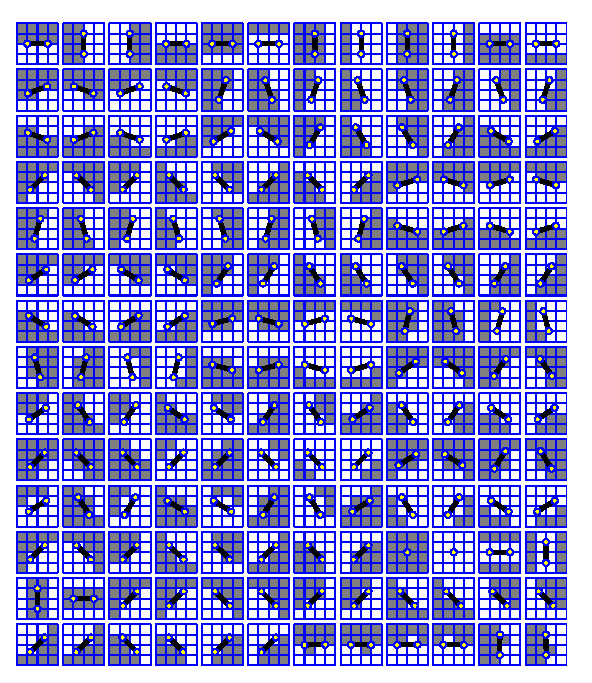
\includegraphics[width=\columnwidth]{seen-all}
\caption{
\label{fig:lines-all}
%
The most frequently observed edge appearances.  All patches
observed are replicated for all $90^{\circ}$ rotations, mirror flips,
and inversion of foreground/background.
%
The most frequent (top) are simple straight edges.
%
The line in the center of
each patch shows the orientation associated with that patch.  
%
After the straight edges, the completely empty patch
is common (produced in saturated regions), 
followed by a tube-like feature (third-last row)
where the boundary is visually distinct to either side of
the edge.
This is followed corner-like features and
many thousands of variations on the themes already seen.  
%
}
\end{center}
\end{figure}
